\begin{figure*}[t]
\centering
% src: fig/abc_slices.png by scripts/paper_figures_abc.py; docs/paper/fig_abc_slices.csv; docs/paper/fig_abc_provenance.json (slices: sections z,y,x = 106, 96, 95; gray range z = -2.18 ... 4.47)
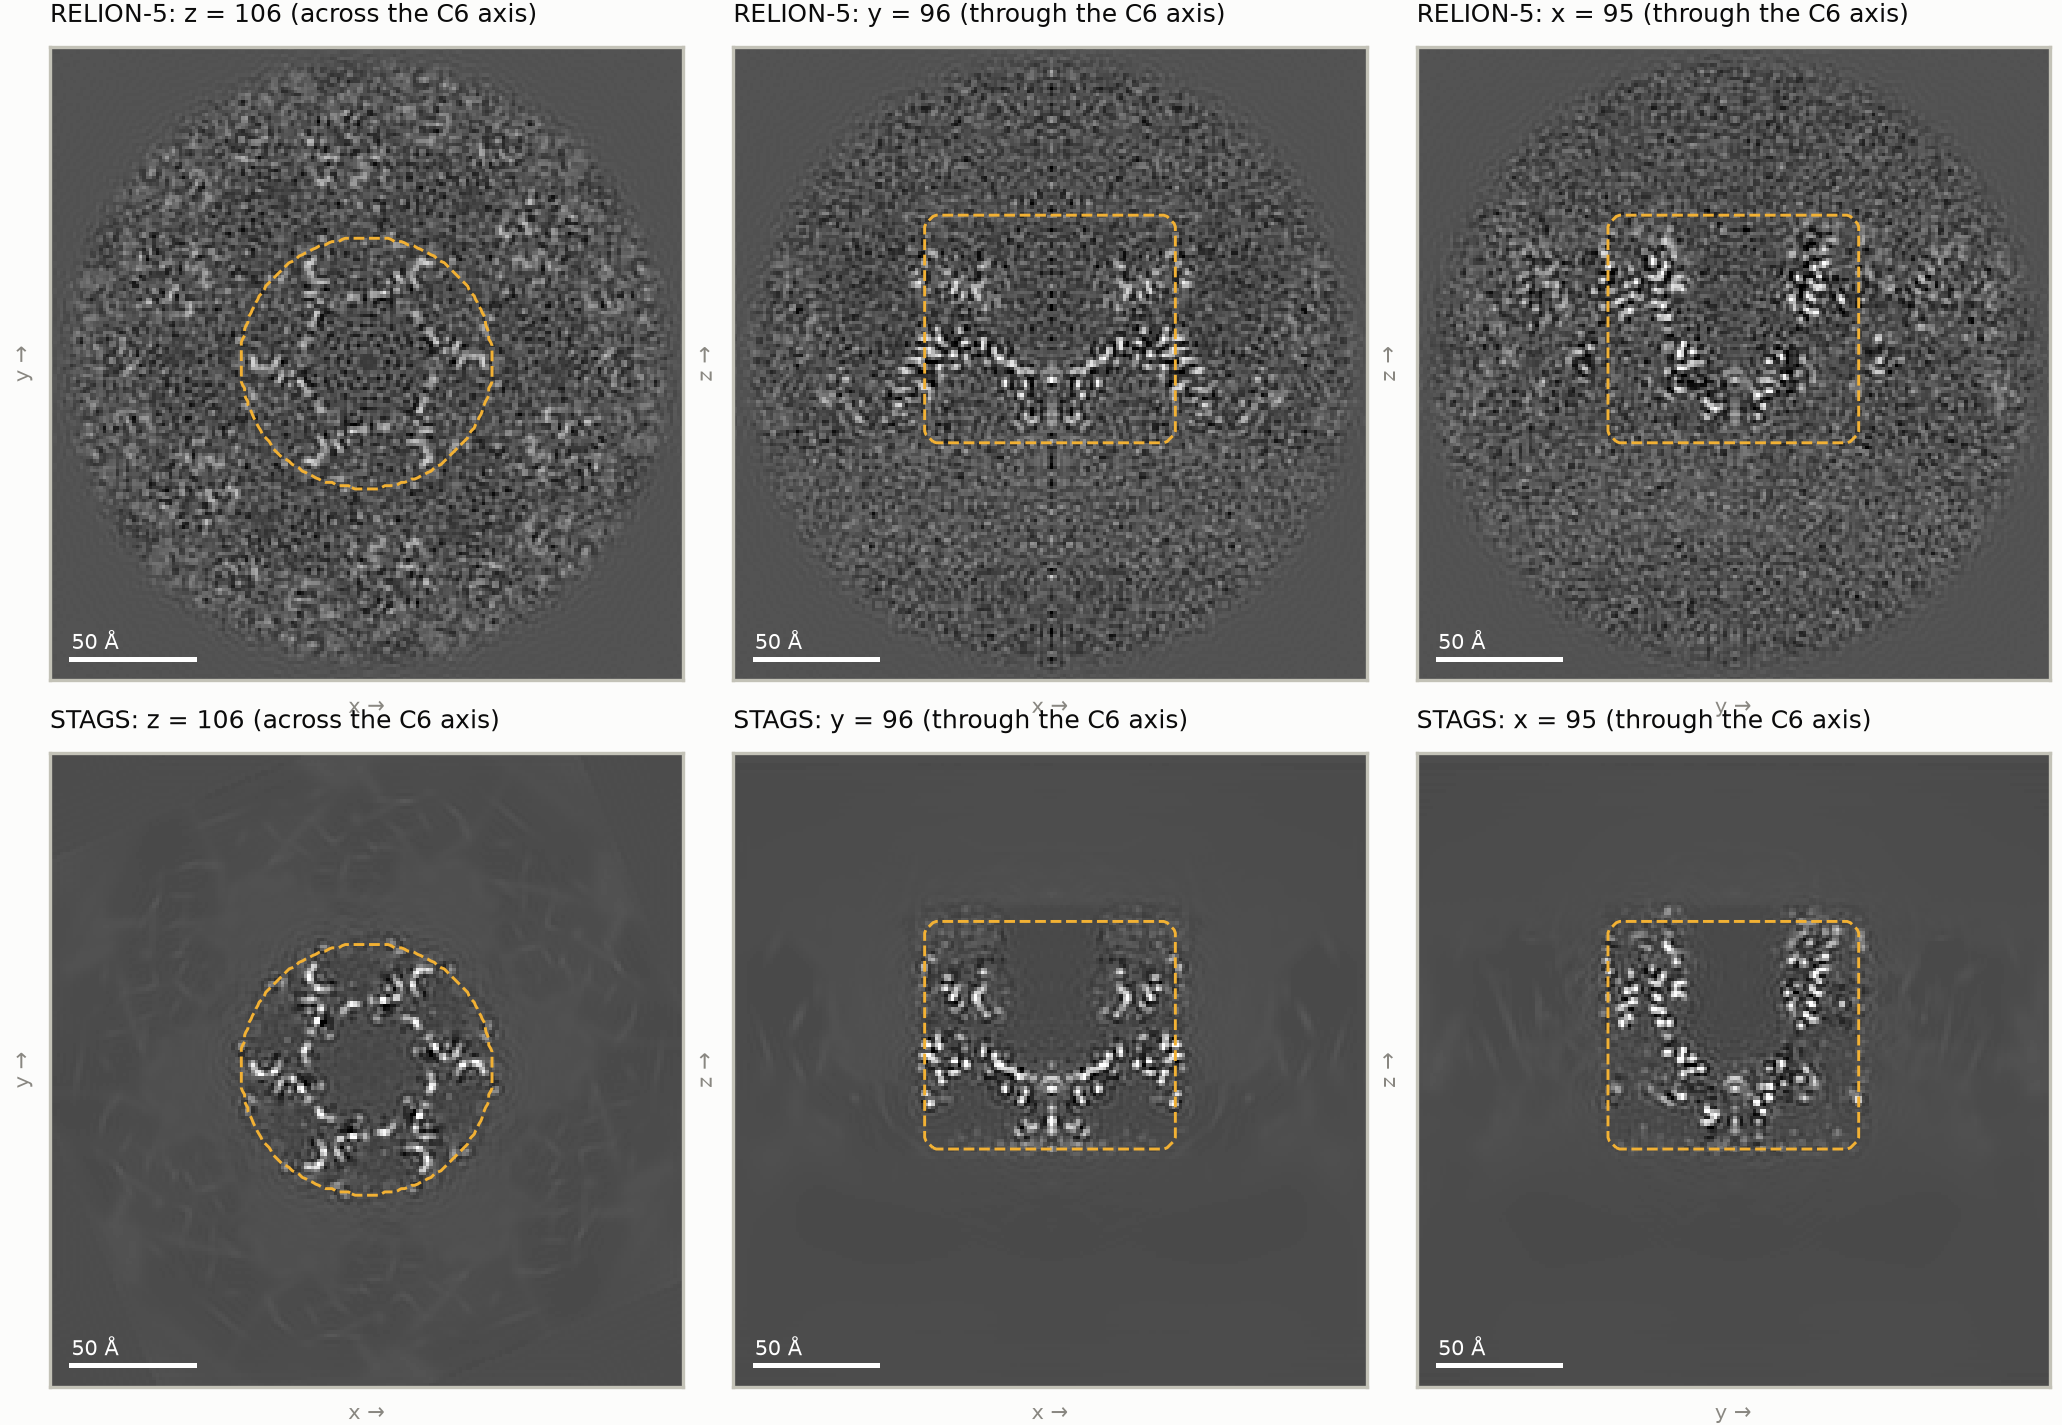
\includegraphics[width=\textwidth]{fig/abc_slices.png}
\caption{\textbf{Central sections, unmasked.}
Top, RELION-5 polished map; bottom, STAGS; one section across and two through the C6 axis.
Same filtering as \cref{fig:views}, z-scored inside RELION's mask (dashed outline), one common gray scale (0.5--99.5\,\% of both maps inside the mask).
Lattice neighbors outside the mask appear only in RELION's map.}
% src: docs/final-campaign-nov13.md (Visual comparison: "STAGS has no density outside its own mask")
\label{fig:slices}
\end{figure*}
